\subsection{Reverse lookup (Enrichr): CNN non-conserved top-200 sets name their own miRNA, beyond site count and expression (positive)}
A stricter use of a target list is to ask whether it identifies its miRNA among thousands. We submit each set to the Enrichr API against the miRTarBase\_2017 library (3,240 miRNA terms; \texttt{scripts/enrichr\_reverse\_lookup.py}; \texttt{results/enrichr\_reverse\_lookup.json}; hermetic tests) and record the rank of the query miRNA's own term by Enrichr's Fisher $p$-value. Panel, sets and seeds match the g:Profiler section. Gates passed: the library's own miR-21-5p set returns miR-21-5p at rank 1; the median random-set own-term rank is 283; all 13 miRNAs are library terms.
H1 is confirmed: CNN top-200 sets rank their own miRNA better than random for 13/13 miRNAs ($p=1.2\times10^{-4}$; median rank 3), and so do CLIP-positive sets (H2, 13/13; partly circular because miRTarBase includes CLIP-derived entries). H3 is falsified: the HEK293 expression top-200 control also ranks the own term well, and the CNN beats it on only 7/13 (4 losses, $p=0.274$).
Because the CNN's univariate CLIP signal was earlier shown to be mostly site-count confounding, and expression dominates the other audits, we added two controls after H1 came back positive (post-hoc, not pre-registered). The CNN beats a site-count top-200 set drawn from the same universe (11 wins, 0 losses, 2 ties, $p=4.9\times10^{-4}$) and random sets matched to the CNN set's expression-decile histogram (13 wins, 0 losses, $p=1.2\times10^{-4}$; Figure~\ref{fig:enrichr}). This is the first audit in the paper where CNN ranking carries signal that survives both confounds.
Limits: miRTarBase 2017 overlaps the miRTarBase 10.0 labels used in the earlier benchmark, so this is a second view of the same kind of evidence rather than an independent one; heavily studied miRNAs (miR-21, miR-155) reach rank 1 even from random sets, so the test carries information mainly for the other 11; and the controls are post-hoc. We record it as a named, falsifiable positive: on a held-out panel with a pre-registered site-count and expression-matched control, CNN top-200 non-conserved sets should keep ranking their own miRNA better than both.
\begin{figure}[h]\centering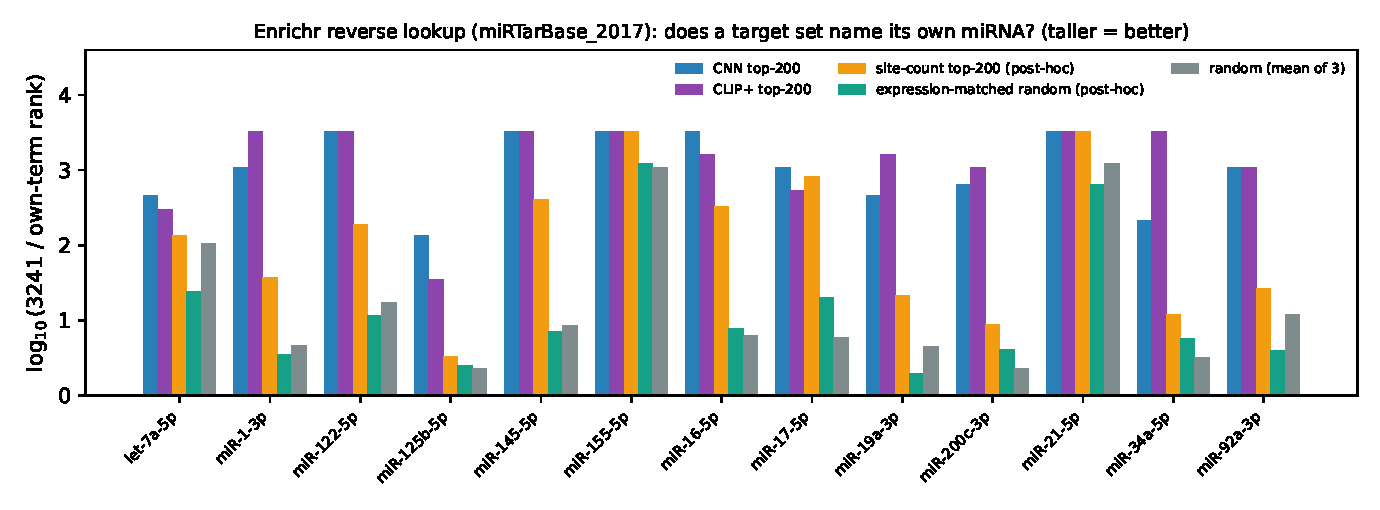
\includegraphics[width=0.95\linewidth]{figs/fig_enrichr.pdf}
\caption{Rank of each miRNA's own miRTarBase\_2017 term when its target set is submitted to Enrichr plotted as $\log_{10}(3241/\mathrm{rank})$, so taller bars mean better ranks. Site-count and expression-matched arms are post-hoc controls.}\label{fig:enrichr}\end{figure}
